\documentclass[runningheads]{llncs}
\usepackage[T1]{fontenc}
\usepackage{newtxtext}
\usepackage[varvw]{newtxmath}
\usepackage{graphicx,booktabs,longtable,xcolor,array}
\usepackage[hidelinks]{hyperref}
\hypersetup{pdfauthor={Dang Truong Minh Le},pdftitle={Supplementary Material: The FundusShift Benchmark}}
\renewcommand\thetable{S\arabic{table}}
\renewcommand\thesection{S\arabic{section}}
\renewcommand\thefigure{S\arabic{figure}}
\emergencystretch=3em
\setlength{\LTcapwidth}{\textwidth}
\newcommand{\G}[1]{\input{generated/supp/#1}}
\newcommand{\reading}[1]{\par\noindent\textit{Reading.} #1\par\medskip}
\begin{document}
\title{Supplementary Material for ``When Fundus Classifiers Meet a New Source: The FundusShift Benchmark and a Low-Capacity Baseline''}
\titlerunning{FundusShift: Supplementary Material}
\author{Dang Truong Minh Le}
\authorrunning{D. T. M. Le}
\institute{Mohamed bin Zayed University of Artificial Intelligence, Abu Dhabi, United Arab Emirates\\ \email{dang.le@mbzuai.ac.ae}}
\maketitle

\noindent This supplement gives every table behind the main paper, plus analyses that did not fit there. All tables are generated from the saved results in the repository (\url{https://doi.org/10.5281/zenodo.23911966}) by \texttt{paper/latex/make\_assets.py}, \texttt{make\_supp.py} and \texttt{make\_supp\_extra.py}; LOTUS is the final method, and the \emph{initial design} is LOTUS with the between-site projection of the main paper (Sec.~5); numbers are means over seeds unless stated. Abbreviations: bAcc, balanced accuracy; Eq-src, mean of per-source bAcc; R/T/F, raw, temperature scaling (TS), focal temperature scaling (FTS); LP, linear probe; LAC, least-ambiguous conformal sets; SGR, selective guaranteed risk; FR, disease images answered normal, over all disease images; G$\to$N, glaucoma images accepted and predicted normal, over all glaucoma images.

\setcounter{tocdepth}{2}
\makeatletter\renewcommand*\l@section{\@dottedtocline{1}{0em}{2.6em}}\makeatother
{\sloppy\tableofcontents}

\section{Data}\label{s:data}
\subsection{Sources, label scope and licences}
Table~\ref{tab:src} lists every source with its class counts per split. ``Scope'' records which diseases a source graded: in DR-only sources a normal label means ``no DR'', and glaucoma was not assessed.
{\tiny\setlength{\tabcolsep}{2.5pt}
\begin{longtable}{@{}lp{.16\textwidth}lllllll@{}}
\caption{Sources. Counts are N/D/G. Development sources contribute train, validation and calibration; test sources and Ch\'ak\d{s}u contribute only the evaluation split.}\label{tab:src}\\
\toprule
Source & Country & Scope & Licence & Train & Validation & Calibration & Test or OOD\\
\midrule\endfirsthead
\caption[]{(continued)}\\
\toprule
Source & Country & Scope & Licence & Train & Validation & Calibration & Test or OOD\\
\midrule\endhead
\G{s1_sources.tex}
\end{longtable}}
\reading{The development side holds 1,395 glaucoma training images, all from Bangladesh Eye (925) and GRAPE (470), whereas DR and normal images come from the six sources other than GRAPE. Five of seven development sources graded only DR. On the test side, only Paraguay is DR-only, HYGD is G-only and PALM is N-only, so per-source bAcc on those two reduces to one recall. These facts explain much of the glaucoma behaviour in the main paper.}

\subsection{Source hierarchy, patients and label scope}
FundusShift holds out whole public \emph{collections} (sources), not hospitals. Table~\ref{tab:hier} gives the institution or country behind each collection, the number of patients where the source releases identifiers, the classes it contributes and what its ``normal'' label means. All but one collection come from a single institution or study; OIA-DDR pools 147 hospitals, so it is one development source with internal variety, not 147 held-out units. Each collection was also assigned an acquisition family (institution), and the audit of Sect.~\ref{s:leak} confirms that no family spans the development and test sides; RFMiD 2.0, from the same institution as IDRiD, is used only for duplicate checks.
\begin{table}[htbp]
\caption{Source hierarchy and label scope. Patients: distinct patient identifiers among used images (n/a: not released; for Ch\'ak\d{s}u only the 60 Bosch-camera images carry identifiers, so its other images form leakage groups by duplicate detection alone and are treated as independent in bootstrap intervals). Normal means: what the source's normal label certifies.}\label{tab:hier}\centering\scriptsize\setlength{\tabcolsep}{3pt}
\begin{tabular}{@{}llp{.28\textwidth}rrll@{}}
\toprule
Role & Source & Institution / country & Images & Patients & Classes & Normal means\\
\midrule
\G{s1_hierarchy.tex}
\end{tabular}
\end{table}
\reading{Five of seven development sources and one test source (Paraguay) graded DR only, so their normal images were never assessed for glaucoma. Only four test sources assessed their normal images for glaucoma (AFIO, FIVES, HRF, which graded all three classes, and PAPILA, which graded N and G); Table~\ref{tab:scopesub} reports test bAcc restricted to them, and the label-scope experiment of Sect.~\ref{s:dev} tests treating DR-only normals as possibly glaucomatous. Because glaucoma appears in only two development sources, glaucoma results measure transfer from those two sites, and the rotations (Table~\ref{tab:gsrc}) show how they change with more glaucoma sources.}

\subsection{Image quality by source}
\begin{table}[htbp]
\caption{Image properties of used images by source (medians): original size, field-of-view fraction, brightness (mean luminance in the field), RMS contrast, Laplacian sharpness, and the share flagged as very dark, overexposed, low field of view or blurry for its source.}\label{tab:quality}\centering\scriptsize\setlength{\tabcolsep}{3pt}
\begin{tabular}{@{}lrrrrrr@{}}
\toprule
Source & Size & FOV & Brightness & Contrast & Sharpness & Flagged\\
\midrule
\G{s1_quality.tex}
\end{tabular}
\end{table}
\reading{Sources differ strongly in resolution, field of view, exposure and sharpness, and these trivial statistics alone identify the source; flagged images are rare (0--3\%). The hardest test sources are not simply the lowest-quality ones: AFIO and FIVES are dark, but Paraguay, the darkest and among the least sharp, is the easiest for every method. Source difficulty therefore reflects class composition and label scope as well as appearance, and we do not attribute it to image quality alone.}

\subsection{Mapping from source labels}
{\scriptsize
\begin{longtable}{@{}llp{.66\textwidth}@{}}
\caption{Native labels mapped to each harmonized class (first token of the stored label; device and vote suffixes omitted).}\label{tab:labels}\\
\toprule
Source & Class & Native labels\\
\midrule\endfirsthead
\caption[]{(continued)}\\
\toprule
Source & Class & Native labels\\
\midrule\endhead
\G{s1_labels.tex}
\end{longtable}}
\reading{A native label is mapped only when it supports the class. Grading scales differ: ICDR grades 1--4, Davis SDR--PDR and named DR categories all become D. Glaucoma suspects in Ch\'ak\d{s}u follow the source's majority vote. HYGD's 199 GON$-$ images were excluded rather than mapped to N, because ``no glaucomatous optic neuropathy'' does not certify the absence of other disease; this makes HYGD single-class. The glaucoma reference standard differs between sources: clinical work-up in GRAPE (visual-field follow-up patients) and HYGD (GON+), image-based expert grading in Ch\'ak\d{s}u (majority vote, including suspects), and not reported for Bangladesh Eye and AFIO, so G pools definitions of different strength. D pools all DR grades from mild NPDR upward; referable DR is not separated (recall by grade: Table~\ref{tab:grade}). The 861-image open-set probe holds images of other conditions from PALM (637), FIVES (200) and AFIO (24), and is distinct from the 860 RFMiD 2.0 images excluded from the core task.}

\subsection{Leakage control and audit}\label{s:leak}
Duplicates were detected by exact SHA-256 hashes and by a vessel-pattern signature (band-pass green channel, $32\times32$) with shift-tolerant normalized cross-correlation at threshold 0.70, then joined with patient identifiers into leakage groups. An automated audit of the released splits found zero violations for each of: a leakage group in more than one split; an identical file in more than one split; a patient in more than one split; a near-duplicate pair across splits; an acquisition family on both development and test sides; a source on both sides; a calibration image without a Cal-A/Cal-B assignment. Brightness-altered copies of GRAPE photographs inside the FIVES glaucoma class were found this way and removed. The detector linked 4,247 image pairs (678 byte-identical, 29 across sources), forming 2,450 leakage groups with more than one image. Of 40,414 inventoried images, 35,280 enter the protocol; the rest were removed for an excluded or unmapped native label (1,820 and 1,453), duplicates whose copies carried conflicting labels (956), a source excluded from the core task (860), or duplication of a test-side image (45). The code is \texttt{fsbench/dedup.py} and \texttt{fsbench/vessel.py}.
\begin{table}[htbp]
\caption{Duplicate links found by the detector (exact hash or vessel-pattern NCC $\ge$ 0.70), by source pair: links, byte-identical links, and links whose two images carry different labels.}\label{tab:dups}\centering\scriptsize
\begin{tabular}{@{}llrrr@{}}
\toprule
Scope & Source(s) & Links & Exact & Label conflict\\
\midrule
\G{s1_duplicates.tex}
\end{tabular}
\end{table}
\reading{All 29 cross-source links join GRAPE photographs to brightness-altered copies inside FIVES, a development--test leak that hashes alone would miss. Within-source links mostly join repeated visits or re-exports; links with conflicting labels concentrate in Bangladesh Eye and Jichi, and the 956 images removed for conflicting labels (above) come from such groups.}

\textbf{Excluded collections.} RFMiD 2.0 was used for inventory and duplicate checks only, because class is confounded with camera. A glaucoma collection of optic-disc crops was excluded for its different field of view. OIA-DDR is CC BY-NC-SA 4.0, so derived data remain non-commercial.

\textbf{Ethics.} All images are publicly released; this is a secondary analysis. Ethics and consent statements were found in the publications of FIVES, GRAPE, PAPILA, SUSTech-SYSU, DeepDRiD, Jichi, HYGD, Ch\'ak\d{s}u, PALM and Paraguay. Statements were not found on the release pages of HRF, Bangladesh Eye and AFIO. Age and sex are available only for PAPILA, so subgroup fairness cannot be assessed.

\section{Models, Recipes and Prompts}\label{s:models}
\begin{table}[htbp]
\caption{Encoders. ``Fine-tuned'' marks the 13 architectures trained end to end; every encoder was also probed frozen.}\label{tab:enc}\centering\scriptsize
\begin{tabular}{@{}llc@{}}
\toprule
Encoder & Pretraining data & Fine-tuned\\
\midrule
\G{s2_encoders.tex}
\end{tabular}
\end{table}

\begin{table}[htbp]
\caption{Training recipes. Every setting selects by validation bAcc unless stated; post-hoc calibration always uses Cal-A, thresholds Cal-B.}\label{tab:recipe}\centering\scriptsize
\begin{tabular}{@{}p{.17\textwidth}p{.79\textwidth}@{}}
\toprule
Fine-tuning & Native input size and normalization; AdamW, lr $10^{-4}$ (head $10^{-3}$), wd 0.05, cosine with one warm-up epoch, 15 epochs, batch 32; (source, class)-balanced sampling; crop, flip, rotation and colour augmentation; mixed precision; five losses (CE; label smoothing 0.1; focal $\gamma{=}3$; MDCA $\beta{=}1$; MbLS $m{=}10$, $\lambda{=}0.1$); 3 seeds. NLL-rule arm: checkpoint by validation NLL.\\
Linear, MLP probes & Frozen embeddings standardized on train; AdamW lr $10^{-3}$, wd $10^{-4}$, 40 epochs, batch 256; weighting none, class or (class, source); MLP: one hidden layer of 512.\\
16-shot probe & 16 images per class, one per leakage group, redrawn per seed, 300 epochs.\\
Zero-shot & Three prompt banks (Table~\ref{tab:prompts}); bank chosen by validation bAcc.\\
CoOp & 16 learnable context tokens, frozen towers, SGD lr 0.002, cosine, 200 full-batch steps on the 16 shots; ctx-init: 4 tokens from ``a photo of a''; CoOp+LP: then a linear head, 200 steps, lr $10^{-3}$; loss variants CE, focal, LS, MbLS, MDCA.\\
Tip-Adapter & Official recipe on the same shots; $(\alpha,\beta)$ grid and bank by validation bAcc (official accuracy rule kept as sensitivity); -F: keys fine-tuned 20 epochs, AdamW lr $10^{-3}$.\\
ERM, Group DRO, CORAL & Fine-tuning recipe with ConvNeXt-T, or DINOv2-B/14 with LoRA rank 8 on query and value; Group DRO $\eta{=}0.01$, group = development source; CORAL $\lambda{=}1$.\\
SWAD & Dense averaging over segments of 150 updates, official loss-valley rule (3, 6, 0.3); replaces the validation checkpoint.\\
WiSE-FT & Head from the zero-shot classifier, AdamW lr $10^{-5}$, wd 0.1, 15 epochs; interpolation $\alpha\in\{0,0.1,\dots,1\}$ chosen by validation bAcc.\\
Multiple choice & Image plus a three-option question; next-token log-likelihoods of the option letters averaged over all six option orders.\\
LOTUS & Table~\ref{tab:spec}.\\
\bottomrule
\end{tabular}
\end{table}

{\scriptsize
\begin{longtable}{@{}lp{.82\textwidth}@{}}
\caption{Prompt banks used by every zero-shot model and by the text branch of LOTUS.}\label{tab:prompts}\\
\toprule
Bank & Prompts\\
\midrule\endfirsthead
\caption[]{(continued)}\\
\toprule
Bank & Prompts\\
\midrule\endhead
\G{s2_prompts.tex}
\end{longtable}}

\section{Complete Benchmark Results}\label{s:all}
{\tiny\setlength{\tabcolsep}{2.4pt}
\begin{longtable}{@{}lllrrrrll@{}}
\caption{Every setting and encoder, with the configuration of highest validation bAcc. $^\dagger$FLAIR's pretraining includes five FundusShift evaluation sources (four test sources and Ch\'ak\d{s}u). Multiple-choice models have no validation scores and no probabilities.}\label{tab:all}\\
\toprule
Setting & Encoder & Config & Val & Test & Eq-src & Ch\'ak\d{s}u & ECE R/T/F & NLL R/T/F\\
\midrule\endfirsthead
\caption[]{(continued)}\\
\toprule
Setting & Encoder & Config & Val & Test & Eq-src & Ch\'ak\d{s}u & ECE R/T/F & NLL R/T/F\\
\midrule\endhead
\G{s3_all.tex}
\end{longtable}}
\reading{Within each setting the encoder ranking on test differs from that on validation (Sect.~\ref{s:rel}). MedSigLIP is the strongest frozen encoder across probe settings, and FLAIR is comparable only on sources it did not see in pretraining. Fine-tuned RETFound reaches high validation (0.886--0.887) but 0.525--0.583 on test, despite fundus pretraining. TS reduces ECE and NLL for most fine-tuned models but leaves ECE far above that of frozen probes. For transparency, the best frozen probe judged by test itself, a class-weighted cross-entropy MedSigLIP linear probe, reached test bAcc 0.778, equal-source 0.702, raw ECE 0.065 and recall G 0.657; validation selected the label-smoothed variant instead.}

\section{Per-Source and Per-Class Results}\label{s:src}
{\scriptsize\setlength{\tabcolsep}{2.6pt}
\begin{longtable}{@{}lrrrrrrrrrr@{}}
\caption{bAcc per unseen source (raw), equal-source mean and worst test source, for LOTUS and the validation-selected representatives.}\label{tab:srcbacc}\\
\toprule
Method & Paraguay & HYGD & FIVES & PAPILA & PALM & HRF & AFIO & Ch\'ak\d{s}u & Eq-src & Worst\\
\midrule\endfirsthead
\caption[]{(continued)}\\
\toprule
Method & Paraguay & HYGD & FIVES & PAPILA & PALM & HRF & AFIO & Ch\'ak\d{s}u & Eq-src & Worst\\
\midrule\endhead
\G{s4_sources.tex}
\end{longtable}}

{\scriptsize\setlength{\tabcolsep}{2.4pt}
\begin{longtable}{@{}lrrrrrrrrrr@{}}
\caption{Class recalls on the multi-class test sources.}\label{tab:recall}\\
\toprule
& \multicolumn{3}{c}{FIVES} & \multicolumn{3}{c}{AFIO} & \multicolumn{2}{c}{PAPILA} & \multicolumn{2}{c}{Paraguay}\\
Method & N & D & G & N & D & G & N & G & N & D\\
\midrule\endfirsthead
\caption[]{(continued)}\\
\toprule
& \multicolumn{3}{c}{FIVES} & \multicolumn{3}{c}{AFIO} & \multicolumn{2}{c}{PAPILA} & \multicolumn{2}{c}{Paraguay}\\
Method & N & D & G & N & D & G & N & G & N & D\\
\midrule\endhead
\G{s4_recall.tex}
\end{longtable}}

{\scriptsize\setlength{\tabcolsep}{2.6pt}
\begin{longtable}{@{}lrrrrrrrrr@{}}
\caption{ECE after TS per source, and the equal-source mean.}\label{tab:srcece}\\
\toprule
Method & Paraguay & HYGD & FIVES & PAPILA & PALM & HRF & AFIO & Ch\'ak\d{s}u & Eq-src\\
\midrule\endfirsthead
\caption[]{(continued)}\\
\toprule
Method & Paraguay & HYGD & FIVES & PAPILA & PALM & HRF & AFIO & Ch\'ak\d{s}u & Eq-src\\
\midrule\endhead
\G{s4_ece.tex}
\end{longtable}}
\begin{table}[htbp]
\caption{LOTUS ECE after TS per source on the published split, three seeds pooled, with 95\% bootstrap intervals over leakage groups (1,000 draws).}\label{tab:ececi}\centering\scriptsize
\begin{tabular}{@{}lrrrl@{}}
\toprule
Source & Images & Groups & ECE (TS) & 95\% CI\\
\midrule
\G{s4_ececi.tex}
\end{tabular}
\end{table}
{\scriptsize\setlength{\tabcolsep}{3pt}
\begin{longtable}{@{}llrlrrrr@{}}
\caption{Per-source accuracy, bAcc, macro-F1 (over classes present) and ECE after TS, three seeds. $^\ast$Single-class source: bAcc equals that class's recall and macro-F1 is degenerate.}\label{tab:persrcfull}\\
\toprule
Method & Source & $n$ & Classes & Acc. & bAcc & Macro-F1 & ECE (TS)\\
\midrule\endfirsthead
\caption[]{(continued)}\\
\toprule
Method & Source & $n$ & Classes & Acc. & bAcc & Macro-F1 & ECE (TS)\\
\midrule\endhead
\G{s4_persource_full.tex}
\end{longtable}}

\begin{figure}[htbp]
\centering
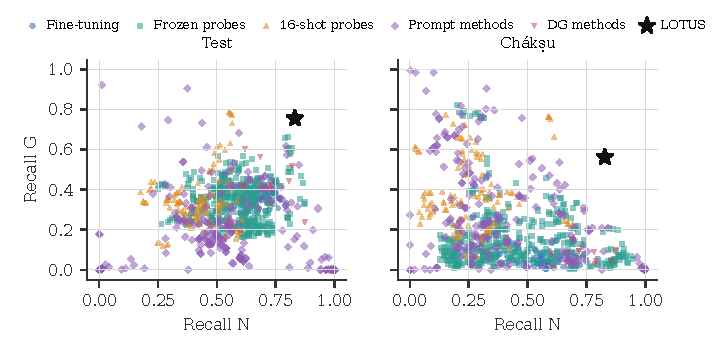
\includegraphics[width=.78\textwidth]{figures/recall.pdf}
\caption{Recall of normal against glaucoma images for every configuration. Few reach the upper right on either view: models either miss glaucoma or over-call it. LOTUS is among the most balanced on test; on Ch\'ak\d{s}u it keeps normal recall high at the cost of glaucoma recall.}\label{fig:recall}
\end{figure}
\begin{table}[htbp]
\caption{Disease-level results, one disease against the rest, after TS, three seeds: sensitivity, specificity, positive predictive value and AUROC.}\label{tab:disease}\centering\scriptsize
\begin{tabular}{@{}lllrrrr@{}}
\toprule
Method & View & Disease & Sens. & Spec. & PPV & AUROC\\
\midrule
\G{s4_disease.tex}
\end{tabular}
\end{table}
\reading{DR is detected well by every method (AUROC 0.93--0.96). Glaucoma separates the methods: LOTUS reaches AUROC 0.926 on test against 0.79--0.87 for the baselines. On Ch\'ak\d{s}u, fine-tuned and DG models detect almost no glaucoma (sensitivity 0.04--0.15); LOTUS has the highest specificity among methods that detect a meaningful share of glaucoma (0.866, sensitivity 0.561, PPV 0.404), whereas the initial design reached sensitivity 0.822 at specificity 0.688. Precision for glaucoma on Ch\'ak\d{s}u stays low for every method, because only 14\% of its images are glaucoma; the higher values of the linear probe and Group DRO (0.50--0.60) come with sensitivities below 0.05.}

\begin{table}[htbp]
\caption{Sensitivity to label scope and single-class sources: test bAcc on all sources, without the single-class HYGD and PALM, and on the four sources that assessed normal images for glaucoma (AFIO, FIVES, HRF, PAPILA; 1,180 images).}\label{tab:scopesub}\centering\scriptsize
\begin{tabular}{@{}lrrr@{}}
\toprule
Method & All test & Without single-class & Full-scope, multi-class\\
\midrule
\G{s4_scope.tex}
\end{tabular}
\end{table}
\reading{On the four sources that graded every class, LOTUS remains first (0.728), ahead of zero-shot (0.689) and the probes (0.608--0.623); every method is lower there than on the pooled test, which Paraguay inflates.}

\reading{Paraguay is easy for every method, whereas AFIO and HRF are hard for all. D transfers well everywhere; the differences between methods come mostly from G and from N on G-heavy sources. Per-source ECE after a single global temperature remains high for every method on HRF and AFIO, small sets where a pooled ECE hides the error. Table~\ref{tab:ececi} shows that their intervals are wide (HRF 0.196--0.438 with 45 images), so calibration on sets this small cannot be certified either way; a deployment site needs a local calibration set of a few hundred images (Table~\ref{tab:budget}).}

\section{Reliability}\label{s:rel}
{\tiny\setlength{\tabcolsep}{2.2pt}
\begin{longtable}{@{}llrrrrrrrrrr@{}}
\caption{Selective prediction on test with thresholds fitted on Cal-B, raw/TS/FTS. Cov~80, Cov~90: thresholds for that coverage on Cal-B. Risk~10: SGR bound of 10\%.}\label{tab:ops}\\
\toprule
& & \multicolumn{4}{c}{Cov 80} & \multicolumn{2}{c}{Cov 90} & \multicolumn{2}{c}{Risk 10} & \multicolumn{2}{c}{Ch\'ak\d{s}u Cov 80}\\
Method & & Cov. & Risk & G$\to$N & D$\to$N & Cov. & Risk & Cov. & Risk & Cov. & Risk\\
\midrule\endfirsthead
\caption[]{(continued)}\\
\toprule
& & \multicolumn{4}{c}{Cov 80} & \multicolumn{2}{c}{Cov 90} & \multicolumn{2}{c}{Risk 10} & \multicolumn{2}{c}{Ch\'ak\d{s}u Cov 80}\\
Method & & Cov. & Risk & G$\to$N & D$\to$N & Cov. & Risk & Cov. & Risk & Cov. & Risk\\
\midrule\endhead
\G{s5_ops.tex}
\end{longtable}}

{\tiny\setlength{\tabcolsep}{2.4pt}
\begin{longtable}{@{}llrrrrrrr@{}}
\caption{Conformal sets on test, quantiles from Cal-B. Coverage/mean size at nominal 0.90; coverage at nominal 0.95.}\label{tab:conf}\\
\toprule
Method & & LAC .90 & APS .90 & Class-LAC .90 & LAC .95 & APS .95 & Class-LAC .95 & Ch\'ak\d{s}u LAC .90\\
\midrule\endfirsthead
\caption[]{(continued)}\\
\toprule
Method & & LAC .90 & APS .90 & Class-LAC .90 & LAC .95 & APS .95 & Class-LAC .95 & Ch\'ak\d{s}u LAC .90\\
\midrule\endhead
\G{s5_conformal.tex}
\end{longtable}}
\reading{Methods whose sets stay near nominal coverage (16-shot, zero-shot) do so with mean set sizes of 1.6 to 1.8 out of three classes, which is of little use. Methods with compact sets lose coverage. TS keeps the ranking of confidence, so it barely changes coverage or risk at a fixed threshold.}

\begin{figure}[htbp]
\centering
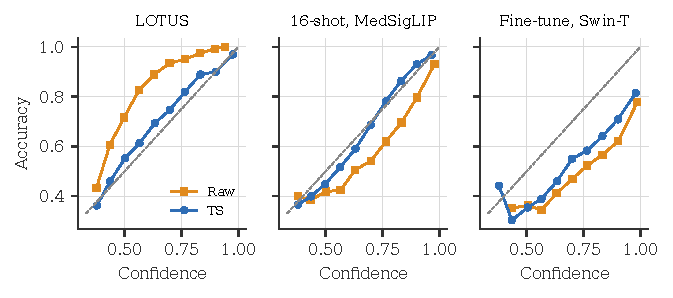
\includegraphics[width=.85\textwidth]{figures/reliability.pdf}
\caption{Test reliability on the published split, seeds pooled, bins with at least 30 images. Raw LOTUS is underconfident and TS brings it near the diagonal; fine-tuned Swin-T stays overconfident after TS.}\label{fig:rel}
\end{figure}

\begin{figure}[htbp]
\centering
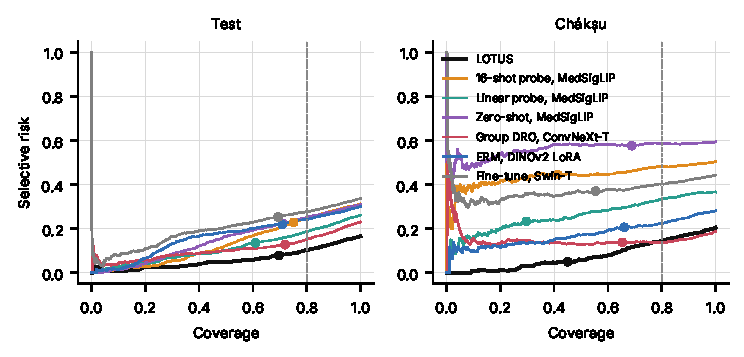
\includegraphics[width=.85\textwidth]{figures/risk_coverage.pdf}
\caption{Risk--coverage curves after TS on the published split (seed 0); dots mark the threshold fitted for 80\% coverage on Cal-B. On Ch\'ak\d{s}u, where 86\% of images are normal, methods that rarely call glaucoma reach low risk while missing most disease.}\label{fig:rc}
\end{figure}
\reading{LOTUS has the lowest area under the risk--coverage curve of every method, on test (0.062; next: linear probe 0.110) and on Ch\'ak\d{s}u (0.081; next: Group DRO 0.269). The Cal-B threshold lands at 69\% coverage instead of 80\%, and on Ch\'ak\d{s}u at 44\%: a threshold fitted on development data does not keep its coverage, and risk alone rewards models that call everything normal.}

\begin{table}[htbp]
\caption{Is the failure caused by too few calibration images? Cal-B is split by leakage group 100 times; thresholds fit on one half are read on the other half (same sources), on test and on Ch\'ak\d{s}u (TS).}\label{tab:halving}\centering\scriptsize\setlength{\tabcolsep}{2.6pt}
\resizebox{\textwidth}{!}{%
\begin{tabular}{@{}lrrrrrrrrr@{}}
\toprule
& \multicolumn{3}{c}{Coverage at Cov 80} & \multicolumn{3}{c}{Risk at Risk 10} & \multicolumn{3}{c}{LAC .90 coverage}\\
Method & Other half & Test & Ch\'ak\d{s}u & Other half & Test & Ch\'ak\d{s}u & Other half & Test & Ch\'ak\d{s}u\\
\midrule
\G{s5_halving.tex}
\end{tabular}}
\end{table}
\reading{On the other half of Cal-B, the promises hold almost exactly; on test and Ch\'ak\d{s}u they fail. The failure therefore comes from the new sources, not from a small calibration set.}

\begin{table}[htbp]
\caption{LOTUS's promises per unseen source on the published split (TS; thresholds fitted on Cal-B): coverage and risk at the thresholds for 80\% and 90\% coverage and at the SGR threshold for risk $\le$ 10\%, and whether that risk target held.}\label{tab:persrcops}\centering\scriptsize
\begin{tabular}{@{}lrrrrrrl@{}}
\toprule
& \multicolumn{2}{c}{Cov 80} & \multicolumn{2}{c}{Cov 90} & \multicolumn{2}{c}{Risk 10} & \\
Source & Cov. & Risk & Cov. & Risk & Cov. & Risk & Held\\
\midrule
\G{s5_persource_ops.tex}
\end{tabular}
\end{table}
\reading{The pooled risk target held (0.086), but per source it held on three of seven test sources (PALM, PAPILA, Paraguay) and on Ch\'ak\d{s}u, and failed on AFIO, FIVES, HRF and HYGD. A pooled guarantee is not a per-site guarantee, and neither is distribution-free under source shift; a deployment site must check its own promises (Table~\ref{tab:target}).}

\clearpage
{\scriptsize
\begin{longtable}{@{}llrrrrrr@{}}
\caption{Calibration budget: fitted $T$ on all of Cal-A, the oracle $T$ fitted on test, and test NLL after TS with natural random subsets of Cal-A (median of 100 draws). $T=1000$ marks the upper bound of the temperature search (zero-shot BiomedCLIP, whose calibrated output is then uniform, NLL $=\ln 3\approx1.10$).}\label{tab:budget}\\
\toprule
Setting & Model & $T$ & $T$ oracle & NLL, 50 & NLL, 200 & NLL, 1000 & NLL, all\\
\midrule\endfirsthead
\caption[]{(continued)}\\
\toprule
Setting & Model & $T$ & $T$ oracle & NLL, 50 & NLL, 200 & NLL, 1000 & NLL, all\\
\midrule\endhead
\G{s5_budget.tex}
\end{longtable}}
\reading{About 200 calibration images give nearly the NLL of the full set, yet the fitted $T$ stays far from the test oracle for several models: more calibration data from the same sources does not close the shift.}

\begin{table}[htbp]
\caption{Trivial predictors, the floor for every metric.}\label{tab:trivial}\centering\scriptsize
\begin{tabular}{@{}llrrrrr@{}}
\toprule
View & Predictor & Acc. & bAcc & Eq-src & ECE & NLL\\
\midrule
\G{s5_trivial.tex}
\end{tabular}
\end{table}
\begin{table}[htbp]
\caption{Spearman correlation between validation and test bAcc across configurations within each setting. Settings with at most two configurations (the four DG methods and the NLL rule, 9 configurations) are not listed separately but are counted in the last row.}\label{tab:rank}\centering\scriptsize
\begin{tabular}{@{}lrr@{}}
\toprule
Setting & Configurations & Spearman\\
\midrule
\G{s5_rank.tex}
\end{tabular}
\end{table}
\reading{A class-prior predictor reaches ECE 0.063 with chance bAcc, so low ECE alone says nothing about usefulness. The high overall rank correlation (0.781 here, over 847 rows that also count the accuracy-rule Tip-Adapter variants; 0.786 over the 816 configurations of the main paper) mostly reflects differences between families; within fine-tuning it is 0.053.}

\section{Robustness Checks}\label{s:rob}
\begin{table}[htbp]
\caption{Fifty random 7/7 source rotations (published split excluded). Probes use class-weighted cross-entropy; arrows go from internal estimates on held-back Cal-B to unseen test sources, after TS.}\label{tab:rot}\centering\scriptsize\setlength{\tabcolsep}{2pt}
\resizebox{\textwidth}{!}{%
\begin{tabular}{@{}lrrrrrrrlll@{}}
\toprule
Method & Val & Test & 5--95\% & Eq-src & Rec.~G & ECE raw & ECE TS & Risk at Cov 80 & LAC .90 & Coverage .80\\
\midrule
\G{s6_rotation.tex}
\end{tabular}}
\end{table}
\reading{Validation exceeded test in 98\% of the 400 probe rows, risk exceeded its internal estimate in 89\%, and LAC fell below its internal coverage in 85\% (338 of 400); for LOTUS the shares were 98\%, 86\% and 92\%. Ranking is not stable either: the 16-shot probe, best on the published split among representatives, is below full training on every encoder over the rotations.}

\begin{table}[htbp]
\caption{Full factorial ablation over the 50 rotations: every combination of bag, between-site projection and text, and text alone; TS, means over three seeds. Last two columns: LOTUS minus the row in bAcc, and rotations where LOTUS is higher.}\label{tab:abl}\centering\scriptsize\setlength{\tabcolsep}{2.2pt}
\resizebox{\textwidth}{!}{%
\begin{tabular}{@{}lrrrrrrrrrrrr@{}}
\toprule
Configuration & bAcc & Macro-F1 & AUROC & Rec.~G & False G & ECE & NLL & AURC & Risk & Ch\'ak\d{s}u & $\Delta$bAcc & Higher\\
\midrule
\G{s6_factorial.tex}
\end{tabular}}
\end{table}
\reading{Every arm with the projection is below the same arm without it (bag + text: 0.789 against 0.771; single head + text: 0.786 against 0.768; bag: 0.779 against 0.754; single head: 0.770 against 0.745), so the projection's cost is consistent rather than an interaction. Text lowers ECE and NLL in every combination; the bag adds little once text is present (0.003) but more without it (0.009 for the single head).}

\begin{table}[htbp]
\caption{Three training seeds per rotation (rotations where all three finished; the probe uses class-weighted cross-entropy as in Table~\ref{tab:rot}). bAcc: mean $\pm$ SD of seed-averaged bAcc across rotations; seed SD: SD across seeds within a rotation, averaged. Last columns: LOTUS minus the row, mean $\pm$ SD over rotations, and rotations where LOTUS has higher bAcc and lower ECE.}\label{tab:seeds}\centering\scriptsize\setlength{\tabcolsep}{3pt}
\begin{tabular}{@{}lrrrrrrrr@{}}
\toprule
Configuration & Rot. & bAcc & Seed SD & ECE & Rec.~G & $\Delta$bAcc & Higher & Lower ECE\\
\midrule
\G{s6_seeds.tex}
\end{tabular}
\end{table}
\reading{Seed variation is an order of magnitude smaller than variation between source partitions, so single-seed rotations measure the partition effect. Against the probe, LOTUS has higher bAcc on 43 and lower ECE on 47 of 50 rotations; text only is better calibrated (lower ECE than LOTUS on 39 of 50) but far less accurate.}

\begin{table}[htbp]
\caption{Why projection hurts. Share of the norm of each class-mean difference that lies in the removed between-site subspace ($k$ directions), on the development data used by each head, against a random subspace of the same size; and alignment between the two glaucoma sites' difference and the N--G direction.}\label{tab:proj}\centering\scriptsize
\begin{tabular}{@{}lrrrrrr@{}}
\toprule
Source left out & $k$ & N--D & N--G & D--G & N--G, random & $|\cos|$ G-site, N--G\\
\midrule
\G{s6_projection.tex}
\end{tabular}
\end{table}
\reading{Fitted on all development data ($k=14$), the between-site directions hold 79--87\% of every class-mean difference; for the individual heads ($k=11$--13) they hold 55--87\%, against 15--23\% for a random subspace of equal size. Sites differ in severity and case mix within each label, so their within-class differences are themselves disease directions; projecting them out removes signal, which explains the accuracy loss over the rotations.}

\begin{table}[htbp]
\caption{How much of the source can be read from each representation. Five-fold cross-validated balanced accuracy of a logistic probe (C = 0.05) predicting the disease, the source, or the source within normal or DR images only, on development (validation and calibration) rows and on test rows. Chance for the source is 1/6 or 1/7.}\label{tab:siteprobe}\centering\scriptsize
\begin{tabular}{@{}llrrrrr@{}}
\toprule
Features & Rows & $n$ & Disease & Source & Source within N & Source within D\\
\midrule
\G{s6_siteprobe.tex}
\end{tabular}
\end{table}
\begin{figure}[htbp]
\centering
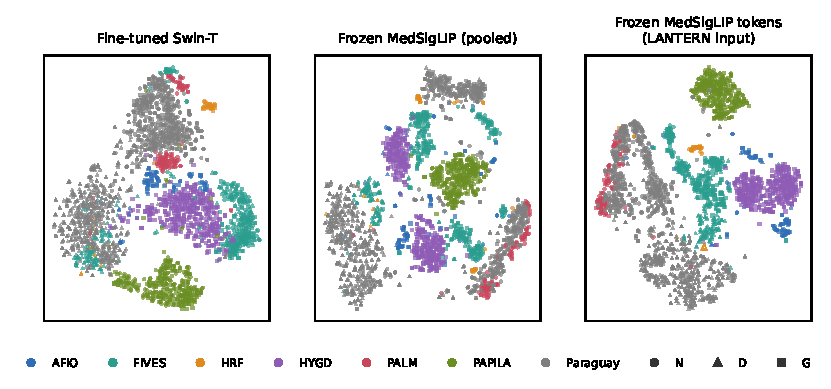
\includegraphics[width=\textwidth]{figures/tsne.pdf}
\caption{t-SNE of test images (2,500 sampled), coloured by source, marker by class, for a fine-tuned encoder and the two frozen MedSigLIP representations. Every representation clusters by source.}\label{fig:tsne}
\end{figure}
\reading{The source is almost perfectly decodable from every representation, frozen or fine-tuned (0.93--1.00), even within one class. Fine-tuning does not add site information, so its failure lies in what its classifier relies on, not in what its features contain; frozen features carry the same site signal, and a low-capacity head simply exploits it less. The between-site projection removes site information for the development sources (0.962 to 0.354) but not for unseen ones (0.998), while it costs disease signal (0.890 to 0.855): it removes the known sites' directions, and new sites differ along new ones.}

\begin{table}[htbp]
\caption{Glaucoma recall over the 50 rotations by the number of development sources that contain glaucoma.}\label{tab:gsrc}\centering\scriptsize
\begin{tabular}{@{}lrrrr@{}}
\toprule
Method & G sources in development & Rotations & Recall G & Test bAcc\\
\midrule
\G{s6_gsrc.tex}
\end{tabular}
\end{table}
\reading{Glaucoma recall grows with the number of glaucoma sources on the development side, so the weakness is one of site diversity, which more sources can address. LOTUS stays ahead of the linear probe at every diversity level observed in more than one rotation (two sources: 0.777 against 0.676; five: 0.788 against 0.772), whereas the initial design fell behind the probe with five sources (0.762 against 0.772).}

\begin{table}[htbp]
\caption{Leave-one-region-out: all non-OOD sources of one region form the test side, the rest the development side (80/10/10 group split), three seeds. Eq-src: mean per-source bAcc; Ch\'ak\d{s}u is read for every split.}\label{tab:region}\centering\scriptsize\setlength{\tabcolsep}{2.4pt}
\resizebox{\textwidth}{!}{%
\begin{tabular}{@{}lp{.3\textwidth}rlrrrrr@{}}
\toprule
Region held out & Test sources & Images & Method & bAcc & Eq-src & Rec.~G & ECE & Ch\'ak\d{s}u\\
\midrule
\G{s6_region.tex}
\end{tabular}}
\end{table}
\reading{Region hold-out is harsher than the rotations for some regions: holding out East Asia removes GRAPE, leaving one glaucoma development source. LOTUS has the highest mean bAcc (0.822), clearly ahead on South Asia (0.751 against 0.678) and the Middle East, within 0.013 of the probe elsewhere, and the best Ch\'ak\d{s}u bAcc in every hold-out; its calibration is not better than the probe's here (mean ECE 0.061 against 0.058).}

\begin{table}[htbp]
\caption{Pairwise AUROC, mean over published test sources holding both classes, with bootstrap intervals over sources.}\label{tab:discrim}\centering\scriptsize
\begin{tabular}{@{}lllrrrrl@{}}
\toprule
Pair & A & B & Sources & AUROC A & AUROC B & A$-$B & 95\% CI\\
\midrule
\G{s6_discrim.tex}
\end{tabular}
\end{table}

\begin{table}[htbp]
\caption{Trained on development sources against trained within the target (logistic regression on frozen features, mean over nine encoders; within-source by cross-validation). Gap: within minus development bAcc, with its bootstrap interval.}\label{tab:ceil}\centering\scriptsize\setlength{\tabcolsep}{2.5pt}
\resizebox{\textwidth}{!}{%
\begin{tabular}{@{}lrrrrrrrrl@{}}
\toprule
& \multicolumn{2}{c}{bAcc} & \multicolumn{2}{c}{ECE} & \multicolumn{2}{c}{AUROC N--G} & \multicolumn{2}{c}{AUROC N--D} & \\
Source & Dev & Within & Dev (TS) & Within & Dev & Within & Dev & Within & Gap\\
\midrule
\G{s6_ceiling.tex}
\end{tabular}}
\end{table}
\reading{N--D and D--G stay near 0.90--0.95 while N--G is 0.64--0.75, so glaucoma is a ranking failure, not a threshold failure. Within-source learning recovers much of it (Ch\'ak\d{s}u gap +0.372), so the labels are learnable and the loss is tied to the shift. AFIO stays low even within source.}

\begin{table}[htbp]
\caption{More training sources at a fixed size (300 images per class): test and Ch\'ak\d{s}u bAcc for $K = 1, 2, 4, 7$ development sources (mean over random pools).}\label{tab:div}\centering\scriptsize
\begin{tabular}{@{}lrrrrrrrr@{}}
\toprule
& \multicolumn{4}{c}{Test} & \multicolumn{4}{c}{Ch\'ak\d{s}u}\\
Encoder & 1 & 2 & 4 & 7 & 1 & 2 & 4 & 7\\
\midrule
\G{s6_sources.tex}
\end{tabular}
\end{table}
\begin{table}[htbp]
\caption{Learning curve: change in test bAcc at $k$ labels per class against the next smaller budget, with bootstrap intervals.}\label{tab:curve}\centering\scriptsize
\begin{tabular}{@{}lrrl@{}}
\toprule
Encoder & $k$ & $\Delta$bAcc & 95\% CI\\
\midrule
\G{s6_curve.tex}
\end{tabular}
\end{table}
\reading{More sources usually help on test (MedSigLIP 0.594 to 0.817 from one to seven sources) but not on Ch\'ak\d{s}u (0.534 to 0.350), and more labels from the same sources give little after about 64 per class. Shift is not solved by more of the same data.}

\section{Attempted Fixes and Other Probes}\label{s:fix}
\begin{table}[htbp]
\caption{Test-time adaptation per held-out source: test bAcc for none, BatchNorm statistics, TENT and T3A ($K$ = 20, 100); Ch\'ak\d{s}u bAcc for none, TENT and T3A-100.}\label{tab:tta}\centering\scriptsize\setlength{\tabcolsep}{3pt}
\begin{tabular}{@{}llrrrrrrrr@{}}
\toprule
Setting & Model & None & BN & TENT & T3A-20 & T3A-100 & Ch.~none & Ch.~TENT & Ch.~T3A\\
\midrule
\G{s7_tta.tex}
\end{tabular}
\end{table}
\begin{table}[htbp]
\caption{Prior correction on top of TS: test bAcc with EM (Saerens et al.) pooled or per source, and with true priors pooled or per source (oracle, uses test labels); ECE for TS, EM per source and oracle per source.}\label{tab:prior}\centering\scriptsize\setlength{\tabcolsep}{2.6pt}
\resizebox{\textwidth}{!}{%
\begin{tabular}{@{}llrrrrrrrr@{}}
\toprule
Setting & Model & TS & EM pooled & EM per src. & True pooled & Oracle per src. & ECE TS & ECE EM & ECE oracle\\
\midrule
\G{s7_prior.tex}
\end{tabular}}
\end{table}
\reading{No label-free fix helps reliably. TENT changes little, BatchNorm adaptation harms ResNet-50 (notably on single-class PALM), and T3A is mostly negative. EM prior estimation is unstable and usually worsens ECE. True per-source priors raise bAcc to 0.81--0.86 for most settings, so class balance is a large part of the shift, but this oracle uses test labels, and single-class sources make it easy.}

{\scriptsize
\begin{longtable}{@{}llrrrrrr@{}}
\caption{$K$ labelled images from each target source, read on the rest of that source: ECE with the frozen $T$ against $T$ re-fitted on $K$; LAC .90 coverage with the frozen quantile against a quantile from $K$, with the 5th percentile over draws.}\label{tab:target}\\
\toprule
Setting & Model & $K$ & ECE frozen & ECE $T$ from $K$ & LAC frozen & LAC from $K$ & LAC 5\%\\
\midrule\endfirsthead
\caption[]{(continued)}\\
\toprule
Setting & Model & $K$ & ECE frozen & ECE $T$ from $K$ & LAC frozen & LAC from $K$ & LAC 5\%\\
\midrule\endhead
\G{s7_target.tex}
\end{longtable}}
\reading{Ten labels from the new source already bring LAC coverage near 0.90 on average and re-fitted $T$ lowers ECE, but the worst draws stay far below nominal at small $K$; this is a deployment recipe, not a guarantee.}

\begin{table}[htbp]
\caption{CLAHE against unprocessed images, same seeds and hardware.}\label{tab:clahe}\centering\scriptsize\setlength{\tabcolsep}{3pt}
\begin{tabular}{@{}lllrrrrrr@{}}
\toprule
Setting & Config & Preprocessing & Val & Test & Eq-src & Ch\'ak\d{s}u & ECE TS & Rec.~G\\
\midrule
\G{s7_clahe.tex}
\end{tabular}
\end{table}
\reading{CLAHE does not help fine-tuning or the 16-shot probe. The MedSigLIP linear probe rises on test, but its validation falls, so validation-based selection would not adopt it.}

\begin{table}[htbp]
\caption{Referral rules at a threshold for 80\% coverage on Cal-B: maximum softmax (MSP), KNN distance in feature space, or both. Open: share of the 861 out-of-scope images accepted.}\label{tab:gate}\centering\scriptsize
\begin{tabular}{@{}lllrrrrr@{}}
\toprule
Setting & Model & Score & Test cov. & Test risk & Cal-B cov. & Open & G$\to$N\\
\midrule
\G{s7_gate.tex}
\end{tabular}
\end{table}
\begin{table}[htbp]
\caption{Out-of-scope detection AUROC from penultimate features of trained models (SWAD rows omitted: its saved checkpoint holds pre-averaging weights).}\label{tab:ood}\centering\scriptsize
\begin{tabular}{@{}llrrrrr@{}}
\toprule
Setting & Model & MSP & MaxLogit & Energy & KNN & Mahalanobis\\
\midrule
\G{s7_ood.tex}
\end{tabular}
\end{table}
\reading{MSP accepts a third to two thirds of out-of-scope images. KNN rejects most of them and lowers risk, but largely by dropping whole hard sources; it is useful for flagging strange images rather than as a remedy for shift.}

\begin{table}[htbp]
\caption{Multiple-choice answering by multimodal LLMs (mean over six option orders).}\label{tab:mcq}\centering\scriptsize
\begin{tabular}{@{}lrrrrrr@{}}
\toprule
Model & Test bAcc & Rec.~N & Rec.~D & Rec.~G & Ch\'ak\d{s}u bAcc & Ch\'ak\d{s}u Rec.~G\\
\midrule
\G{s7_mcq.tex}
\end{tabular}
\end{table}
\begin{table}[htbp]
\caption{Recall of D by DR grade on test (grade $-1$: Davis grading without a numeric ICDR grade).}\label{tab:grade}\centering\scriptsize
\begin{tabular}{@{}llrrrrr@{}}
\toprule
Setting & Model & $-1$ & 1 & 2 & 3 & 4\\
\midrule
\G{s7_grade.tex}
\end{tabular}
\end{table}
\begin{table}[htbp]
\caption{Glaucoma recall on clean test images and at the strongest blur and JPEG levels.}\label{tab:deg}\centering\scriptsize
\begin{tabular}{@{}llrrr@{}}
\toprule
Setting & Model & Clean & Blur & JPEG\\
\midrule
\G{s7_degrade.tex}
\end{tabular}
\end{table}
\reading{Generative multimodal models rarely call glaucoma. Mild DR (grade 1) is the hardest D grade for most models. Strong blur, and for most models JPEG compression, mainly remove glaucoma recall, consistent with the disc being a small, detail-dependent region; the 16-shot MedSigLIP probe is the exception under JPEG (0.784 to 0.870).}

\section{LOTUS: Specification and Development}\label{s:dev}
\begin{table}[htbp]
\caption{Complete specification of LOTUS. The initial design adds the projection row before the heads.}\label{tab:spec}\centering\scriptsize
\begin{tabular}{@{}lp{.76\textwidth}@{}}
\toprule
Encoder & MedSigLIP (patch 14, 448 px, 27 layers, width 1152), frozen\\
Head input & Last hidden state, $32\times32$ tokens pooled to $14\times14$; fixed random orthonormal map to 384 dimensions (seed 0); grid mean\\
Standardization & Per dimension, training-split mean and standard deviation\\
Projection & None. Initial design only: within-class between-site means, at most 32 directions (their rank gives 11--13 per head, 14 on all development data), fitted per head on its training rows\\
Heads & One linear head per development source, trained without it; 1,155 parameters each\\
Training & Label smoothing 0.1; class-balanced sampling; AdamW, lr $3\times10^{-4}$, wd $10^{-2}$; batch 64; 12 epochs; best epoch by validation bAcc on the head's own sites\\
Rescaling & Centre per image; divide by the standard deviation over validation rows\\
Text & Mean of the three banks of Table~\ref{tab:prompts}, on the pooled image embedding\\
Fusion & 0.5 heads + 0.5 text; TS on Cal-A\\
Seeds & 0, 1, 2 on the published split and on every rotation; the main rotation table uses seed 0 for all methods\\
\bottomrule
\end{tabular}
\end{table}

\subsection{Design search on development sources}
The design search below produced the initial design; LOTUS removes its projection after the rotation ablation (Table~\ref{tab:abl}). All results in this section are leave-one-development-source-out on development data, equal-site mean, three seeds unless noted, and use no test row. Table~\ref{tab:gate7} compares losses (cross-entropy; a conditional-logit pair loss across sites, ``cross''; the same within sites, ``strata''), a single head against a leave-one-source-out bag, the between-site projection (``nap''), and text fusion with one bank or all three, on pooled MedSigLIP features.
{\scriptsize
\begin{longtable}{@{}lrrrr@{}}
\caption{Factorial comparison on pooled features (development, three seeds).}\label{tab:gate7}\\
\toprule
Arm & bAcc & ECE & NLL & Recall G\\
\midrule\endfirsthead
\caption[]{(continued)}\\
\toprule
Arm & bAcc & ECE & NLL & Recall G\\
\midrule\endhead
\G{s8_gate7.tex}
\end{longtable}}
\reading{Every component adds a little alone; with all three in place the loss choice no longer matters (0.791--0.794). Text with all banks is the largest single step.}

{\scriptsize
\begin{longtable}{@{}llrrrrr@{}}
\caption{Head input (pooled feature, last-layer token mean, three depths, both) and head recipe (base: 40 epochs, lr $10^{-3}$, wd $10^{-4}$, batch 256; reg: 12 epochs, lr $3\times10^{-4}$, wd $10^{-2}$, batch 64), single head or bag with projection, with text.}\label{tab:inputs}\\
\toprule
Study & Arm & bAcc & ECE & NLL & Recall G & False G\\
\midrule\endfirsthead
\caption[]{(continued)}\\
\toprule
Study & Arm & bAcc & ECE & NLL & Recall G & False G\\
\midrule\endhead
\G{s8_inputs.tex}
\end{longtable}}

\begin{table}[htbp]
\caption{Initial design on each held-out development site.}\label{tab:devsites}\centering\scriptsize
\begin{tabular}{@{}lrrr@{}}
\toprule
Held-out site & bAcc & Recall G & False G\\
\midrule
\G{s8_dev_sites.tex}
\end{tabular}
\end{table}

\begin{table}[htbp]
\caption{Designs tried and not retained (development). Reference: pooled-feature pipeline 0.791; single cross-entropy head 0.675.}\label{tab:neg}\centering\scriptsize
\begin{tabular}{@{}p{.46\textwidth}rp{.42\textwidth}@{}}
\toprule
Experiment & bAcc & Reading\\
\midrule
Batch network predicting temperature and class bias (1 seed) & .539 & Below the raw head (.666)\\
EM prior shift with TS (1 seed) & .523 & Unreliable with few classes per source\\
Polar Fourier features around the disc & .702 & Below the pair loss alone (.723)\\
Site prior, $\kappa$ from 30 to 3000 & .693--.717 & No gain\\
Full residual corrector over logits & .667 & Recall G fell to 0\\
Corrector with fusion weights only & .781 & ECE .057, bAcc did not rise\\
RPAttn head on three token depths (1 seed) & .664 & Recall G .008; with text .690\\
RPAttn + MixStyle (1 seed) & .614 & Recall G .012; with text .688\\
N/D from RPAttn, G from low-capacity branch (1 seed) & .788 & .793 for the pooled pipeline on that seed\\
Late fusion of nine encoder inputs & .765 & Other encoders lowered the score\\
Greedy nested encoder selection & .789 & Mostly kept MedSigLIP alone\\
Magnified optic-disc view with whole image & .768 & Recall G up (.767), false G up (.135)\\
Image-conditioned fusion gate & .763 & Below a plain average\\
Global class offset chosen on other sites & .679 & GRAPE fell to .006\\
ConvNeXt-T end-to-end with pair loss (1 seed) & .622 & GRAPE .004\\
\bottomrule
\end{tabular}
\end{table}
\reading{Heavier or learned modules repeatedly lost the glaucoma class at held-out sites, which led to the low-capacity design.}

\subsection{Error analysis and disc-side bias}
\begin{table}[htbp]
\caption{Held-out development sites for the pooled-feature pipeline: head, text and fusion bAcc, recalls, and images wrong under all nine encoder inputs.}\label{tab:err}\centering\scriptsize
\begin{tabular}{@{}lrrrrrrrr@{}}
\toprule
Held-out site & $n$ & Head & Text & Fusion & N & D & G & All wrong\\
\midrule
Bangladesh Eye & 3,153 & .651 & .732 & .753 & .761 & .963 & .536 & .039 \\
OIA-DDR & 11,269 & .660 & .738 & .735 & .685 & .786 & -- & .137 \\
DeepDRiD & 1,804 & .803 & .721 & .795 & .682 & .908 & -- & .111 \\
GRAPE & 528 & .644 & .750 & .741 & -- & -- & .741 & .104 \\
IDRiD & 462 & .757 & .752 & .751 & .527 & .974 & -- & .100 \\
Jichi & 8,475 & .779 & .736 & .803 & .824 & .781 & -- & .103 \\
SUSTech-SYSU & 1,097 & .975 & .889 & .957 & .938 & .975 & -- & .009 \\
\bottomrule

\end{tabular}
\end{table}
\reading{On OIA-DDR, 1,629 of 5,639 normal images were predicted G although the source holds no glaucoma. Between 0.9\% and 13.7\% of a site's images were wrong under all nine inputs; among normal IDRiD images, 28\%. A global class offset did not fix the G confusion, so it is a ranking problem.}

\begin{table}[htbp]
\caption{Normal images predicted G, by disc side (automatic, label-free disc location), held-out site.}\label{tab:side}\centering\scriptsize
\begin{tabular}{@{}lrr@{}}
\toprule
Held-out site & Disc left & Disc right\\
\midrule
OIA-DDR & .386 & .191\\
Bangladesh Eye & .141 & .023\\
IDRiD & .119 & .045\\
SUSTech-SYSU & .086 & .019\\
Jichi & .067 & .054\\
DeepDRiD & .096 & .086\\
\bottomrule
\end{tabular}
\end{table}

{\scriptsize
\begin{longtable}{@{}lrrrrrr@{}}
\caption{Upgrades of the initial design's input on development data: dimension (384 or 1152), mirrored training and averaging, NAP $k$, weight decay. A separate study with its own runs; its ``d384 plain'' baseline is the initial design's configuration but differs slightly from the main development ablation (0.789 against 0.792).}\label{tab:upg}\\
\toprule
Arm & bAcc & NLL & Recall G & False G & N$\to$G left & N$\to$G right\\
\midrule\endfirsthead
\caption[]{(continued)}\\
\toprule
Arm & bAcc & NLL & Recall G & False G & N$\to$G left & N$\to$G right\\
\midrule\endhead
\G{s8_upgrade.tex}
\end{longtable}}
\reading{Mirroring removes the left-right gap and lowers false G but costs recall G; all 1152 dimensions are worse; $k$ and weight decay hardly matter.}

\begin{table}[htbp]
\caption{Post-processing checked on held-out development sites, fitted on calibration rows of the other sites.}\label{tab:post}\centering\scriptsize\setlength{\tabcolsep}{3pt}
\begin{tabular}{@{}lrrrrrrrrl@{}}
\toprule
State & ECE & NLL & Cov~80 cov. & Cov~80 risk & Risk~10 risk & LAC cov. & LAC size & Class-LAC & APS cov./size\\
\midrule
\G{s8_post.tex}
\end{tabular}
\end{table}

\clearpage
\subsection{Patch-level evidence}
The head input is the mean of patch tokens, and standardization, projection and the linear head are all linear, so each head's logits split exactly into per-patch contributions: $z_s(x)=\frac{1}{P}\sum_p W_s(I-U_sU_s^{\top})x_p+b_s$ for the initial design, and the same without the projection for LOTUS. The maps below were computed with the initial design. Figure~\ref{fig:evidence} maps the glaucoma evidence (G logit minus the larger of N and D, averaged over heads) for the most and least confident glaucoma image of each glaucoma test source. Tokens recomputed for these images matched the stored ones to within 0.13 (feature scale about 90).
\begin{figure}[htbp]
\centering
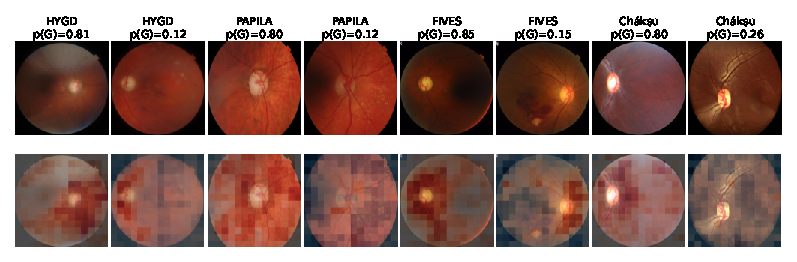
\includegraphics[width=\textwidth]{figures/evidence.pdf}
\caption{Glaucoma evidence per patch (red: for G, blue: against), for the most and least confident glaucoma image of each source, $p(\mathrm{G})$ from raw fused logits. In confident cases the evidence concentrates on the optic disc; in missed cases it is weak and diffuse. Text scores are global and not mapped.}\label{fig:evidence}
\end{figure}
\reading{The maps are exact decompositions of the head, not post-hoc saliency, but they are not a validated localization of pathology.}

\subsection{Failure cases}
\begin{figure}[htbp]
\centering
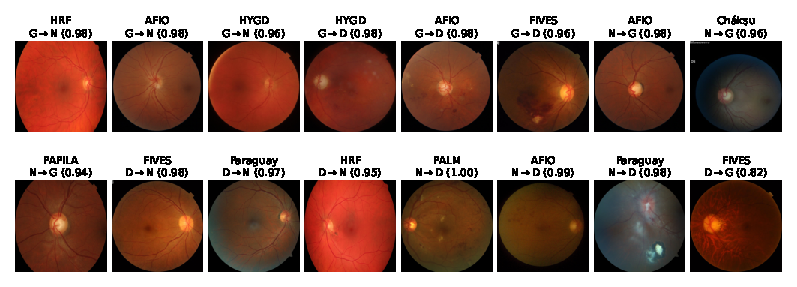
\includegraphics[width=\textwidth]{figures/failures.pdf}
\caption{Most confident errors of the initial design on test and Ch\'ak\d{s}u (seed 0, after TS), up to three sources per error type: true$\to$predicted class and confidence.}\label{fig:fail}
\end{figure}
\reading{Errors are often confident (0.82--1.00 after TS), which a global temperature cannot catch. Three patterns recur. Glaucoma missed as normal or DR occurs on sources with strong colour casts or low contrast (HRF, AFIO), where the disc is less distinct. Normal images called glaucoma show a prominent, bright disc. Normal or DR confusions on Paraguay and PALM involve visible bright or dark spots in images labelled normal, which may reflect label scope (Paraguay graded only DR) rather than model error; without re-grading we cannot tell. These observations are descriptive, not a clinical review.}

\subsection{Later attempts}
Two further components were tried with selection rules written before their results were read; label scope was tested with the initial design, and the shift-aware reference is reported for LOTUS (Table~\ref{tab:cert}; the initial design kept the risk target on 44 of 50 rotations against 23). \emph{Label scope}: normal labels from DR-only sources were treated as the set \{N, G\}, with likelihood $p_\mathrm{N}+p_\mathrm{G}$. \emph{Shift-aware reference}: temperature, thresholds and conformal quantiles were fitted on leave-one-source-out predictions rather than on Cal-B, with an optional normal certificate.
\begin{table}[htbp]
\caption{Label scope, tested with the initial design: development (scope-aware bAcc counts a DR-only normal predicted G as correct) and the 50 rotations.}\label{tab:scope}\centering\scriptsize
\begin{tabular}{@{}lrrrrrr@{}}
\toprule
Arm & bAcc & Scope-aware bAcc & ECE & Recall G & N$\to$G, DR-only & N$\to$G, full scope\\
\midrule
\G{s8_scope.tex}
\end{tabular}
\end{table}
{\scriptsize
\begin{longtable}{@{}llrrlrrrr@{}}
\caption{LOTUS thresholds from Cal-B against the leave-one-source-out reference, 50 rotations, with and without the normal certificate; Held: rotations where test risk stayed at or below 10\%. Cal-B is used whole, as in Table~9 of the paper (same values); the rotation table of the paper (Table~5) fits on one half of Cal-B and reads the other, so its LOTUS values differ in the third decimal.}\label{tab:cert}\\
\toprule
Fitted on & Target & Test cov. & Test risk & Held & FR & G$\to$N & Ch\'ak\d{s}u cov. & Ch\'ak\d{s}u risk\\
\midrule\endfirsthead
\caption[]{(continued)}\\
\toprule
Fitted on & Target & Test cov. & Test risk & Held & FR & G$\to$N & Ch\'ak\d{s}u cov. & Ch\'ak\d{s}u risk\\
\midrule\endhead
\G{s8_cert.tex}
\end{longtable}}
\reading{Label scope over-calls glaucoma at new sources. The shift-aware reference keeps coverage and risk promises far more often; risk at matched coverage is identical for both, so the arms differ only in where the threshold sits.}

\section{Statistical Comparisons}\label{s:stat}
{\scriptsize
\begin{longtable}{@{}llrrrr@{}}
\caption{Paired bootstrap over leakage groups on the published split, 2,000 draws, Holm within each metric; differences are LOTUS minus baseline. Adjusted $p=0.009$ is the floor set by 2,000 draws after Holm correction. Intervals are conditional on these seven test sources and on LOTUS's test-based selection; they do not include source-level variance (bAcc SD 0.039 across rotations).}\label{tab:paired}\\
\toprule
Metric & Baseline & Baseline value & Diff. & 95\% CI & Adj. $p$\\
\midrule\endfirsthead
\caption[]{(continued)}\\
\toprule
Metric & Baseline & Baseline value & Diff. & 95\% CI & Adj. $p$\\
\midrule\endhead
bAcc (raw) & 16-shot probe, MedSigLIP & .748 & +0.082 & [+0.067, +0.097] & 0.009 \\
bAcc (raw) & Linear probe, MedSigLIP & .728 & +0.102 & [+0.088, +0.116] & 0.009 \\
bAcc (raw) & Zero-shot, MedSigLIP & .709 & +0.122 & [+0.107, +0.136] & 0.009 \\
bAcc (raw) & ERM, DINOv2 LoRA & .707 & +0.123 & [+0.107, +0.138] & 0.009 \\
bAcc (raw) & Group DRO, ConvNeXt-T & .707 & +0.124 & [+0.109, +0.138] & 0.009 \\
bAcc (raw) & Fine-tune (NLL rule), ConvNeXt-T & .677 & +0.154 & [+0.136, +0.170] & 0.009 \\
bAcc (raw) & CORAL, ConvNeXt-T & .676 & +0.154 & [+0.137, +0.170] & 0.009 \\
bAcc (raw) & SWAD, ConvNeXt-T & .672 & +0.158 & [+0.141, +0.175] & 0.009 \\
bAcc (raw) & Fine-tune, Swin-T & .655 & +0.176 & [+0.157, +0.193] & 0.009 \\
bAcc (raw) & WiSE-FT, SigLIP2-L & .634 & +0.196 & [+0.177, +0.214] & 0.009 \\
bAcc (raw) & MLP probe, DINOv2-B & .598 & +0.232 & [+0.213, +0.250] & 0.009 \\
bAcc (raw) & CoOp ctx-init, BiomedCLIP & .497 & +0.334 & [+0.315, +0.352] & 0.009 \\
bAcc (raw) & CoOp + LP, SigLIP-B & .496 & +0.335 & [+0.316, +0.353] & 0.009 \\
bAcc (raw) & Tip-Adapter-F, BiomedCLIP & .495 & +0.336 & [+0.315, +0.356] & 0.009 \\
bAcc (raw) & CoOp, SigLIP-B & .491 & +0.339 & [+0.320, +0.357] & 0.009 \\
bAcc (raw) & Tip-Adapter, BiomedCLIP & .478 & +0.352 & [+0.332, +0.373] & 0.009 \\
\midrule
ECE (TS) & Zero-shot, MedSigLIP & .032 & -0.002 & [-0.017, +0.013] & 0.799 \\
ECE (TS) & 16-shot probe, MedSigLIP & .044 & -0.014 & [-0.026, -0.000] & 0.091 \\
ECE (TS) & Linear probe, MedSigLIP & .079 & -0.050 & [-0.066, -0.028] & 0.009 \\
ECE (TS) & Group DRO, ConvNeXt-T & .091 & -0.062 & [-0.078, -0.043] & 0.009 \\
ECE (TS) & Tip-Adapter, BiomedCLIP & .091 & -0.062 & [-0.076, -0.044] & 0.009 \\
ECE (TS) & ERM, DINOv2 LoRA & .115 & -0.086 & [-0.103, -0.066] & 0.009 \\
ECE (TS) & Fine-tune (NLL rule), ConvNeXt-T & .133 & -0.104 & [-0.121, -0.081] & 0.009 \\
ECE (TS) & CORAL, ConvNeXt-T & .136 & -0.107 & [-0.124, -0.084] & 0.009 \\
ECE (TS) & SWAD, ConvNeXt-T & .139 & -0.109 & [-0.127, -0.087] & 0.009 \\
ECE (TS) & Tip-Adapter-F, BiomedCLIP & .147 & -0.118 & [-0.135, -0.100] & 0.009 \\
ECE (TS) & CoOp ctx-init, BiomedCLIP & .150 & -0.121 & [-0.140, -0.099] & 0.009 \\
ECE (TS) & WiSE-FT, SigLIP2-L & .168 & -0.139 & [-0.156, -0.117] & 0.009 \\
ECE (TS) & Fine-tune, Swin-T & .171 & -0.142 & [-0.158, -0.119] & 0.009 \\
ECE (TS) & MLP probe, DINOv2-B & .172 & -0.143 & [-0.160, -0.119] & 0.009 \\
ECE (TS) & CoOp, SigLIP-B & .175 & -0.146 & [-0.164, -0.124] & 0.009 \\
ECE (TS) & CoOp + LP, SigLIP-B & .176 & -0.147 & [-0.164, -0.124] & 0.009 \\
\midrule
NLL (TS) & 16-shot probe, MedSigLIP & .644 & -0.187 & [-0.212, -0.162] & 0.009 \\
NLL (TS) & Zero-shot, MedSigLIP & .690 & -0.234 & [-0.254, -0.214] & 0.009 \\
NLL (TS) & Linear probe, MedSigLIP & .694 & -0.238 & [-0.271, -0.202] & 0.009 \\
NLL (TS) & Group DRO, ConvNeXt-T & .926 & -0.469 & [-0.536, -0.405] & 0.009 \\
NLL (TS) & ERM, DINOv2 LoRA & .944 & -0.487 & [-0.552, -0.430] & 0.009 \\
NLL (TS) & CORAL, ConvNeXt-T & 1.005 & -0.549 & [-0.613, -0.487] & 0.009 \\
NLL (TS) & Tip-Adapter, BiomedCLIP & 1.020 & -0.563 & [-0.592, -0.533] & 0.009 \\
NLL (TS) & Fine-tune (NLL rule), ConvNeXt-T & 1.036 & -0.579 & [-0.650, -0.513] & 0.009 \\
NLL (TS) & SWAD, ConvNeXt-T & 1.056 & -0.599 & [-0.672, -0.529] & 0.009 \\
NLL (TS) & Tip-Adapter-F, BiomedCLIP & 1.099 & -0.643 & [-0.679, -0.608] & 0.009 \\
NLL (TS) & Fine-tune, Swin-T & 1.174 & -0.717 & [-0.790, -0.645] & 0.009 \\
NLL (TS) & CoOp + LP, SigLIP-B & 1.180 & -0.723 & [-0.777, -0.669] & 0.009 \\
NLL (TS) & CoOp, SigLIP-B & 1.180 & -0.724 & [-0.776, -0.671] & 0.009 \\
NLL (TS) & CoOp ctx-init, BiomedCLIP & 1.189 & -0.733 & [-0.789, -0.675] & 0.009 \\
NLL (TS) & WiSE-FT, SigLIP2-L & 1.243 & -0.787 & [-0.863, -0.711] & 0.009 \\
NLL (TS) & MLP probe, DINOv2-B & 1.259 & -0.802 & [-0.897, -0.708] & 0.009 \\
\bottomrule

\end{longtable}}

\begin{table}[htbp]
\caption{Configurations with development bAcc of at least 0.791, all evaluated on the published split; the one with the highest test bAcc (bold) became the initial design, and LOTUS is this configuration without the projection. Values are from the selection run; the re-run used everywhere else (Table~7 of the paper) gives the initial design 0.815, recall G 0.753 and Ch\'ak\d{s}u 0.733. All ten exceed the best test bAcc of any validation-selected representative (0.748).}\label{tab:cand}\centering\scriptsize
\resizebox{\textwidth}{!}{%
\begin{tabular}{@{}lrrrrrr@{}}
\toprule
Configuration & Dev & Test bAcc & Eq-src & Recall G & NLL (TS) & Ch\'ak\d{s}u\\
\midrule
Mirror, weight decay $10^{-3}$ & .800 & .809 & .726 & .696 & .503 & .714 \\
Mirror, weight decay $10^{-2}$ & .799 & .808 & .727 & .708 & .502 & .726 \\
Mirror, weight decay $10^{-4}$ & .795 & .807 & .724 & .681 & .511 & .703 \\
Cross-site pair loss & .794 & .809 & .717 & .722 & .507 & .694 \\
Same-site pair loss & .792 & .791 & .696 & .670 & .524 & .713 \\
\textbf{Tokens, weight decay $10^{-2}$ (selected)} & .792 & .817 & .724 & .765 & .482 & .731 \\
Pooled feature, weight decay $10^{-4}$ & .791 & .799 & .706 & .687 & .520 & .684 \\
Pooled feature + tokens & .791 & .812 & .719 & .719 & .493 & .701 \\
Disc side canonicalised & .791 & .805 & .733 & .679 & .511 & .637 \\
Mirrored text only & .791 & .800 & .714 & .679 & .512 & .704 \\
\bottomrule

\end{tabular}}
\end{table}


\subsection{Follow-up: clean selection, input versus recipe, prior correction, screening}\label{s:followup}
All on the 50 rotations (\texttt{experiments/extra\_runs.py}, \texttt{results/extra}).
\begin{table}[h]\caption{Follow-up results, means over rotations. Nested: arm chosen per rotation by leave-one-source-out on development only (LOTUS 29, initial design 8, single head + text 7, other 6). EM: label-free prior correction per test source.}\label{tab:followup}\centering\scriptsize
\begin{tabular}{lcccc}\toprule
Model & bAcc & ECE (TS) & bAcc after EM & ECE after EM\\\midrule
Nested selection (no held-out data) & 0.780 & 0.035 & -- & --\\
LOTUS (tokens) & 0.789 & 0.034 & 0.732 & 0.210\\
LOTUS on pooled features & 0.789 & 0.035 & 0.737 & 0.204\\
LOTUS head recipe, pooled, no bag/text & 0.763 & 0.055 & 0.720 & 0.220\\
Probe recipe on tokens & 0.752 & 0.077 & 0.755 & 0.176\\
Linear probe (pooled) & 0.746 & 0.084 & 0.750 & 0.182\\\bottomrule
\end{tabular}\end{table}
\reading{Selecting without held-out data costs 0.009 and keeps the lead over the probe (39 of 50) and the calibration gain (47 of 50). The recipe and text, not the token input, carry the gain. Prior correction helps no model reliably and ruins calibration.}

\textbf{Simple baselines} (\texttt{experiments/review\_baselines.py}, \texttt{results/review\_baselines}; 50 rotations, seed 0, same splits and evaluation). The rotation linear probe fused 1/2 + 1/2 with LOTUS's text scores reached bAcc 0.777, ECE 0.043, NLL 0.534 and recall G 0.666; LOTUS (0.788, 0.034, 0.508, 0.708) was ahead by $0.012\pm0.021$ (higher on 35 of 50; ECE lower on 33). One LOTUS head on all development sources, six seeds averaged, plus text, reached 0.786, ECE 0.035 and recall G 0.695; LOTUS was ahead by $0.002\pm0.007$ (27 of 50).
\reading{Added to the probe, text fusion gives 0.745 to 0.777 and the head recipe 0.777 to 0.788; removed from LOTUS, text costs 0.010 and the recipe more (Table~\ref{tab:abl}), so the split depends on the order. The leave-one-source-out construction adds no more than seed averaging. LOTUS is best read as a regularized linear-head ensemble fused with zero-shot text.}

\textbf{Recipe components} (\texttt{experiments/recipe\_ablation.py}, \texttt{results/recipe\_ablation}). One head on all development sources plus text (0.786, within 0.002 of LOTUS), one component changed at a time, 50 rotations, seed 0.
\begin{table}[h]\centering\scriptsize\caption{Head recipe ablation. Reference: smoothing 0.1, class-balanced resampling, 12 epochs, AdamW lr $3\cdot10^{-4}$, weight decay $10^{-2}$, best epoch by validation bAcc. Last column: rotations where the reference is higher.}\label{tab:recipe}
\begin{tabular}{@{}lrrrrrr@{}}\toprule
Variant & bAcc & $\Delta$ & ECE & NLL & Recall G & Ref.\ higher\\\midrule
\G{s9_recipe.tex}
\end{tabular}\end{table}
\reading{Class-balanced resampling carries most of the recipe, mainly through recall G; less training (fewer steps, lower learning rate) helps, consistent with low capacity; smoothing and weight decay do not matter. The 4-epoch variant is better but was found after the fact and is not adopted.}

\textbf{Screening thresholds.} Thresholds on $P(G)$ set on Cal-B for 90\% specificity gave, over rotations, test specificity 0.837 and sensitivity 0.857 for LOTUS (probe: 0.789 and 0.860), but on Ch\'ak\d{s}u specificity 0.336 at sensitivity 0.954 (probe: 0.622 and 0.637). On the published split, 95\% specificity on Cal-B gave 0.882 on test with sensitivity 0.798 (probe 0.865 and 0.708). Specificity targets, like risk targets, do not hold at new sources and must be set locally.

\section{External Cohorts}\label{s:ext}
\textbf{Protocol.} Written on 5 November 2026, before any external image was scored (\texttt{docs/protocol\_external.md}; code \texttt{experiments/external.py}; results \texttt{results/external}).
Messidor-2: 1,744 gradable images with adjudicated ICDR grades (Krause et al., Ophthalmology 2018) (public Hugging Face copy \texttt{sngsfydy/Messidor2}); grade 0 $\to$ N, 1--4 $\to$ D, as in the benchmark; its normals are DR-only normals. G1020: 1,020 images, 724 normal and 296 glaucoma ($\to$ G); no DR grading. Both are reported separately, never pooled, because class and source coincide within each.
Images were cropped and resized as the benchmark images. Models: LOTUS and the initial design (seeds 0--2; heads refit with the original seeds on the published split; every benchmark logit matched \texttt{results/revision/final} exactly), MedSigLIP zero-shot, ConvNeXt-T with CE and with Group DRO (seeds 0--2, saved checkpoints). Feature extraction reproduced the stored arrays on 64 benchmark images (maximum absolute difference: mean tokens 0.0013, fp16 rounding; pooled features and zero-shot logits $<10^{-5}$; ConvNeXt logits $\le$ 0.026). Temperature on Cal-A; the 80\% coverage threshold and 90\% LAC quantile on the same half of Cal-B as in the paper; specificity thresholds on all of Cal-B.
\textbf{Overlap.} Nearest benchmark image by pooled MedSigLIP cosine: at most 0.953 (Messidor-2) and 0.968 (G1020); no pair above 0.95 was a pHash near copy, so no image was removed. MedSigLIP's fundus pretraining data is EyePACS; neither cohort is listed.

\begin{table}[h]
\caption{External cohorts, frozen published-split models (mean of 3 seeds; zero-shot: 1), evaluated once after TS on Cal-A. Messidor-2: 1,017 N, 727 D (ICDR 1--4); G1020: 724 N, 296 G. FG/FD: share predicted as the class absent from the cohort. AUROC: disease vs normal ($1-p(\mathrm{N})$); Ref.: referable DR (ICDR $\ge$ 2).}\label{tab:ext}
\centering\scriptsize\setlength{\tabcolsep}{2.8pt}
\begin{tabular}{@{}lrrrrrrrrrrr@{}}
\toprule
& \multicolumn{7}{c}{Messidor-2 (France, DR)} & \multicolumn{4}{c}{G1020 (Germany, glaucoma)}\\
\cmidrule(lr){2-8}\cmidrule(l){9-12}
Model & bAcc & Rec.\,D & FG & AUROC & Ref. & ECE & LAC & bAcc & Rec.\,G & FD & AUROC\\
\midrule
\G{s10_ext.tex}
\end{tabular}
\end{table}

\begin{table}[h]\centering\scriptsize\setlength{\tabcolsep}{3pt}
\caption{External cohorts, further metrics (mean of 3 seeds). Spec./Sens.: at the Cal-B threshold on $p(\cdot)$ of the cohort's disease for 90\% and 95\% specificity (Cal-B specificity 0.899 for every model). Cov./Risk: at the 80\% coverage threshold. Published-test ECE for reference.}\label{tab:ext2}
\begin{tabular}{@{}llrrrrrrrrrrrr@{}}\toprule
Cohort & Model & Rec.\,N & D1 & D2 & D3 & D4 & Cov. & Risk & NLL & Sp.90 & Se.90 & Sp.95 & Se.95\\\midrule
\G{s10_ext2.tex}
\end{tabular}\end{table}
D1--D4: recall D by ICDR grade on Messidor-2 (mild DR is the hard grade for every model). Seed standard deviation of bAcc: LOTUS 0.011 (Messidor-2) and 0.005 (G1020); ConvNeXt-T 0.008--0.039. Paired bootstrap of bAcc (2,000 resamples, seed-averaged probabilities), LOTUS minus comparator: Messidor-2, initial design $-0.019$ [$-0.029$, $-0.009$], zero-shot +0.026 [0.008, 0.043], CE $-0.003$ [$-0.026$, 0.021], Group DRO +0.031 [0.007, 0.055]; G1020, initial design 0.000 [$-0.009$, 0.008], zero-shot +0.055, CE +0.052, Group DRO +0.043 (all intervals above 0), differences between models that all sit at chance AUROC.
$^*$From \texttt{experiments/review\_baselines.py}: the linear probe of the rotations (class-weighted cross-entropy on pooled features), refit on the published split with seeds 0--2, alone and fused 1/2 + 1/2 with the same text scores as LOTUS; same TS and evaluation; LAC and FD were not computed for them. This probe reaches bAcc 0.791 on the published test split, above the validation-selected linear-probe representative (0.728, Table~7 of the paper), so it is a strong comparator. Paired bootstrap intervals use seed-averaged probabilities, so they need not equal differences of the seed-mean bAcc in the table.

\textbf{Is G1020 learnable at all?} As a diagnostic (no model of the paper is changed), a logistic regression on the same frozen MedSigLIP tokens was trained and tested within each cohort by 5-fold cross-validation (5 repetitions, three regularization strengths; \texttt{experiments/external\_learnability.py}). Messidor-2 DR vs normal reached AUROC 0.89--0.93; G1020 glaucoma vs non-glaucoma reached 0.46--0.47. G1020's labels are therefore not recoverable from these image features even with in-cohort training; on inspection its non-glaucoma class includes eyes with other retinal findings, which explains the many DR predictions. G1020 is a test of label definition rather than of glaucoma transfer, and glaucoma transfer to non-Asian populations remains untested.
\reading{DR transfers in ranking and calibration but not in decisions: normals are over-called, as glaucoma (14\% of all images predicted G) or DR, and coverage and LAC promises fail as at the test sources. The plain probe ranks DR as well as LOTUS but is worse calibrated; fused with text it matches LOTUS on Messidor-2.}

\textbf{Label-free site standardization (negative).} Rules written before the run (\texttt{docs/protocol\_site\_adapt.md}; \texttt{experiments/site\_adapt.py}): token features of each site standardized with that site's own mean and std, from its images and no labels (the frozen-feature analogue of AdaBN), either at unseen sites only (heads unchanged) or at every source (heads refit). Adoption required higher mean bAcc than LOTUS on at least 30 of 50 rotations. Over the 50 rotations (seed 0), bAcc fell from 0.788 to 0.685 (unseen sites only) and 0.692 (every source), lower on all 50; recall G fell from 0.708 to 0.394 and 0.442; ECE after TS was 0.055 and 0.034 (LOTUS 0.034). Neither variant is adopted. On the external cohorts (exploratory; seen before the idea) it raised Messidor-2 bAcc to 0.737 and 0.718 at unchanged AUROC (0.82), a shift of the decision bias rather than of the ranking, and left G1020 at chance (AUROC 0.50). A site's own mean carries its class mix, so standardizing it away removes disease signal, as the between-site projection did.

\section{Reproducibility}\label{s:repro}
\sloppy
Code, saved result tables and this document are archived at \url{https://doi.org/10.5281/zenodo.23911966} (GitHub: \url{https://github.com/dangaura-tech/fundusshift}). The README maps each result to its script and table file. LOTUS and its ablation over the rotations and regions are produced by \texttt{experiments/revision\_runs.py} (saved in \texttt{results/revision}); its published-split evaluation and paired tests by \texttt{experiments/lotus\_eval.py}, its rotation promises by \texttt{experiments/lotus\_rotation.py}, the external cohorts by \texttt{experiments/external.py}, and its per-source and disease-level tables by \texttt{experiments/review\_tables.py} (saved in \texttt{results/lotus}). The evaluation protocol, including the selection rules written before each later attempt, is \texttt{docs/protocol.md}. The benchmark (images under their source licences, split table, leakage groups and duplicate lists) is public at \url{https://huggingface.co/datasets/le-dang1haha/FundusShift}; its \texttt{metadata/splits\_final.csv} is the exact split used here.
\end{document}
